\documentclass[conference]{IEEEtran}
\IEEEoverridecommandlockouts

\usepackage{cite}
\usepackage{amsmath,amssymb,amsfonts}
\usepackage{algorithmic}
\usepackage{algorithm}
\usepackage{graphicx}
\usepackage{textcomp}
\usepackage{xcolor}
\usepackage{booktabs}
\usepackage{multirow}
\usepackage{url}
\usepackage{tikz}
\usetikzlibrary{shapes.geometric, arrows.meta, positioning, fit, calc, backgrounds}
\def\BibTeX{{\rm B\kern-.05em{\sc i\kern-.025em b}\kern-.08em
    T\kern-.1667em\lower.7ex\hbox{E}\kern-.125emX}}

\begin{document}

\title{Tackling Extreme Class Imbalance in Wildfire Segmentation: A Combined Loss and Data-Centric Approach\\}

\author{\IEEEauthorblockN{1\textsuperscript{st} Muhammmad Adrean Karim Syauqy}
\IEEEauthorblockA{\textit{School of Electrical Engineering} \\
\textit{Telkom University}\\
Bandung, Indonesia \\
madreans@student.telkomuniversity.ac.id}
\and
\IEEEauthorblockN{2\textsuperscript{nd} I Kadek Nuary Trisnawan}
\IEEEauthorblockA{\textit{School of Electrical Engineering} \\
\textit{Telkom University}\\
Bandung, Indonesia \\
ikadeknuarytrisnawan@telkomuniversity.ac.id}
\and
\IEEEauthorblockN{3\textsuperscript{rd} Hasbi Ash Shiddiqey}
\IEEEauthorblockA{\textit{School of Electrical Engineering} \\
\textit{Telkom University}\\
Bandung, Indonesia \\
hasbisiddiq@telkomuniversity.ac.id}
\and
\IEEEauthorblockN{4\textsuperscript{th} Rifqi M. Fikri}
\IEEEauthorblockA{\textit{School of Electrical Engineering} \\
\textit{Telkom University}\\
Bandung, Indonesia \\
rifqmff@telkomuniversity.ac.id}
\and
\IEEEauthorblockN{5\textsuperscript{th} Daffa Khusnureza}
\IEEEauthorblockA{\textit{School of Electrical Engineering} \\
\textit{Telkom University}\\
Bandung, Indonesia \\
daffaunu@student.telkomuniversity.ac.id}
\and
\IEEEauthorblockN{6\textsuperscript{th} Stevanus Wahyu Julianto}
\IEEEauthorblockA{\textit{School of Electrical Engineering} \\
\textit{Telkom University}\\
Bandung, Indonesia \\
stevan@student.telkomuniversity.ac.id}
}

\maketitle

\begin{abstract}
Automated detection of fire and smoke via remote camera networks is critical for mitigating the impact of wildfires. While semantic segmentation models offer precise pixel-level boundaries, their deployment is severely hindered by extreme dataset imbalances. In wildfire imagery, the target objects occupy a minuscule fraction of the high-resolution frame, and there exists a drastic intra-class imbalance where diffuse smoke heavily outnumbers active flame fronts. In this paper, we empirically demonstrate that naive segmentation pipelines catastrophically fail on the minority flame class, achieving a mere 62.1\% Fire mIoU on the FIgLib dataset. To solve this, we propose an optimization pipeline centered on a custom Combined Loss formulation (Lovasz-Softmax, Focal, and Dice) that explicitly rescues the minority class, boosting Fire mIoU to 79.9\%. Furthermore, we introduce secondary data-centric optimizations---namely, an RGCr color space transformation and a Balanced SAHI-style Tiling algorithm---that force the network to prioritize the thermal signatures of active flames over diffuse smoke. Our ablation studies reveal a critical trade-off: while the Combined Loss alone yields the highest overall accuracy (79.9\% Fire+Smoke mIoU), appending our RGCr and Tiling strategies successfully pushes Fire mIoU to a state-of-the-art 81.1\%, sacrificing a fraction of smoke boundary precision to guarantee the detection of critical combustion events.
\end{abstract}

\begin{IEEEkeywords}
Semantic Segmentation, Wildfire Detection, Class Imbalance, Combined Loss, PIDNet, Color Space, Tiling
\end{IEEEkeywords}

\section{Introduction}
The rapid proliferation of camera-based remote surveillance systems has positioned computer vision as the vanguard technology for early wildfire detection. Unlike rudimentary object detection bounding boxes, semantic segmentation classifies images at the pixel level, providing precise morphological boundaries. This pixel-level accuracy is critical for downstream disaster management systems, as it enables the extraction of vital physical parameters—such as the volume of the fire, the vector of propagation, and the rate of spread—which are essential for deploying first responders effectively.

However, deploying segmentation models in the wild introduces severe, often debilitating, data-centric problems. The fundamental issue is extreme class imbalance, which manifests in two distinct ways. First, there is a drastic foreground-background imbalance. In high-resolution remote camera imagery, the objects of interest (fire and smoke) occupy a minuscule fraction of the total pixel space compared to the vast background (e.g., sky, foliage, mountains). Second, and more critically, there is a severe intra-class imbalance: diffuse smoke is far more prevalent, voluminous, and visible than the active flame front itself. In our analyzed subset of the FIgLib (Fire Image Library) dataset, this intra-class disparity manifests as a staggering 1:7 Fire-to-Smoke annotation ratio.

When standard training methodologies and loss functions (like Cross-Entropy) are applied to such imbalanced datasets, deep learning models invariably fall into a statistical trap. The model rapidly learns to minimize global loss by becoming highly proficient at classifying the majority classes (background and smoke) while functionally ignoring the minority class (active flames). This results in a model that boasts high overall accuracy but is functionally useless for its primary task: detecting the actual fire. Furthermore, standard data loading practices exacerbate this problem. High-resolution surveillance imagery is typically downsampled to fit GPU memory constraints, a process that permanently destroys the high-frequency spatial features of early-stage, microscopic flame fronts.

In this paper, we propose a comprehensive, problem-driven methodology to solve these class imbalance and resolution challenges. Utilizing the highly efficient Proportional-Integral-Derivative Network (PIDNet) \cite{pidnet} as our baseline architecture, our empirical results demonstrate that architectural choices alone are insufficient. Instead, we propose a heavily optimized data and loss pipeline.

The primary contributions of this paper are:
\begin{itemize}
    \item We demonstrate that a custom Combined Loss strategy (synergizing Lovasz-Softmax, Focal Loss, and Dice Loss with aggressive class weighting) is the singular most effective intervention for extreme imbalance, single-handedly boosting Fire mIoU from 62.1\% to 79.9\%.
    \item We introduce an RGCr (Red, Green, Chrominance-Red) color space transformation and a deterministic Balanced Tiling algorithm to combat resolution loss and prioritize the thermal signatures of active flames over diffuse smoke.
    \item We present comprehensive ablation studies on the FIgLib dataset, providing actionable insights into the precision-recall trade-offs required for life-critical disaster monitoring systems.
\end{itemize}

\section{Related Work}

\subsection{Wildfire Detection and Segmentation}
Early visual detection of wildfires relied on hand-crafted thresholds for color and texture, which were highly susceptible to false positives from clouds and sun glare. While the shift toward deep learning significantly improved generalization, modern models still acutely struggle with false positives caused by low-altitude clouds, fog, and atmospheric haze \cite{govil2020preliminary, nguyen2023smokeynet}. Furthermore, the requirement for edge processing on remote cameras has driven the adoption of highly efficient architectures like BiSeNet and PIDNet, which balance spatial resolution with fast inference speeds. However, these lightweight networks are particularly vulnerable to extreme class imbalance and the "small object problem"---where early-stage fires occupy merely a handful of pixels---as they lack the massive parameter counts required to memorize complex minority class distributions.

\subsection{Addressing Class Imbalance}
Class imbalance is a pervasive issue in computer vision. At the data level, techniques like oversampling or SMOTE are commonly used, though they are difficult to apply to dense segmentation masks. At the algorithmic level, custom loss functions have proven highly effective. Focal Loss \cite{focal} modifies Cross-Entropy to dynamically down-weight "easy" background examples. The Lovasz-Softmax loss \cite{lovasz} provides a smooth, differentiable surrogate for the discrete Jaccard index (IoU), allowing networks to directly optimize for set overlap regardless of class frequency.

\subsection{Handling Small Objects and Color Spaces}
To counteract the "small object problem" caused by downsampling high-resolution imagery, Slicing Aided Hyper Inference (SAHI) \cite{sahi} is often employed to infer on high-resolution overlapping patches. Additionally, researchers have found success manipulating color spaces (e.g., YCbCr, or HSV \cite{muhammad2023fire}) to isolate the luminance and chrominance signatures of combustion, preventing the network from confusing white smoke with clouds.

\subsection{Basic Segmentation Architecture (PIDNet)}
Unlike conventional segmentation architectures that often sacrifice boundary details for semantic context, PIDNet \cite{pidnet} was introduced to provide an optimal balance. Inspired by Proportional-Integral-Derivative (PID) controllers, this network employs a three-branch architecture designed to simultaneously process spatial details (Proportional), high-level semantic context (Integral), and object boundaries (Derivative). This three-branch design makes it uniquely suited for preserving the sharp, microscopic boundaries of early-stage fires---an area where encoder-decoder networks like UNet traditionally struggle---while maintaining high efficiency for processing high-resolution imagery. However, as demonstrated in this paper, while PIDNet is inherently strong at preserving boundary details, it still requires specific loss and data-level adaptations when faced with extreme class imbalances.

\subsection{Data Sources}
Early research on wildfire detection heavily relied on small-scale datasets or irregularly curated internet images. As deep learning approaches evolved, several dedicated databases emerged, such as the Corsican Fire Database and the FLAME dataset, providing video and thermal imagery. However, for training semantic segmentation models that require highly precise pixel-level boundaries in wildland conditions, the FIgLib (Fire Image Library) provided by HPWREN has become one of the most comprehensive sources. This dataset includes high-resolution imagery from remote cameras in real-world conditions, which, despite its value, introduces significant challenges in the form of extreme class imbalance among smoke, fire, and background.

\section{Methodology}
\label{sec:methodology}

Our proposed methodology addresses the failures of naive segmentation pipelines through a two-pronged approach: a custom Combined Loss strategy to combat class imbalance at the gradient level, and a set of data-centric optimizations (Temporal Pruning, Color Space Transformation, and Balanced Tiling) designed to prioritize the thermal signatures of the flame front over diffuse smoke.

\begin{figure}[htbp]
\centering
\resizebox{\columnwidth}{!}{%
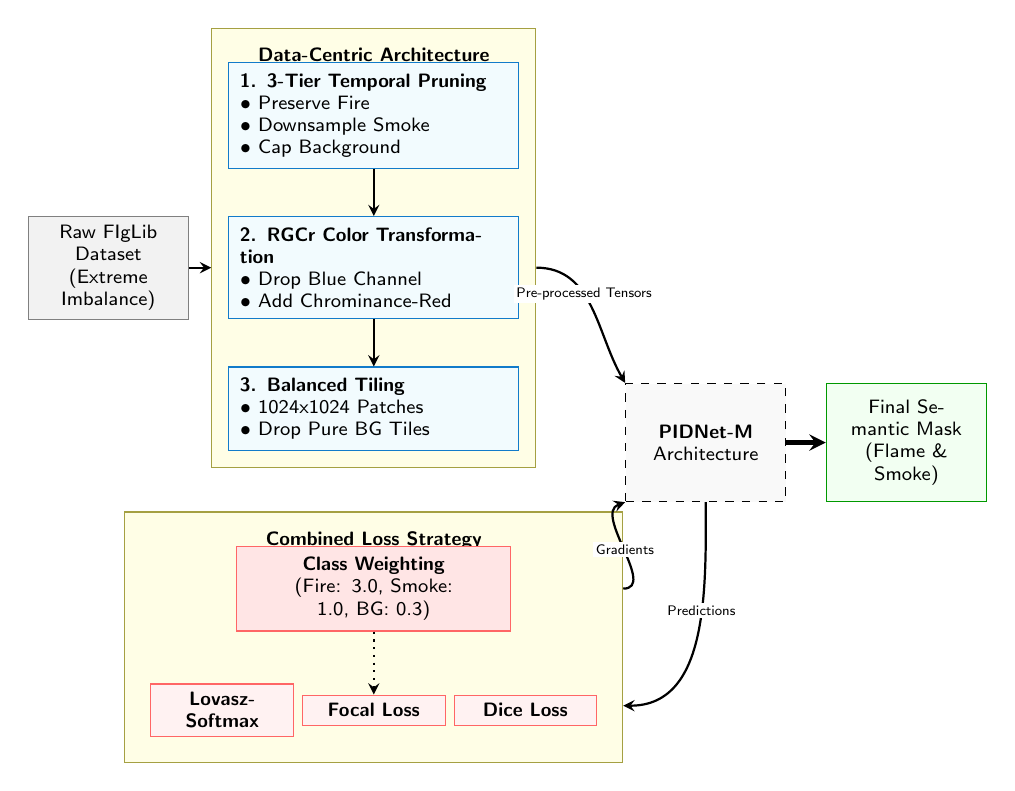
\begin{tikzpicture}[
    node distance=0.6cm and 0.5cm,
    font=\sffamily\scriptsize,
    >=stealth,
    % Styles
    raw/.style={rectangle, draw=gray, fill=gray!10, text width=1.8cm, align=center, minimum height=1.2cm},
    datablock/.style={rectangle, draw=cyan!60!blue, fill=cyan!5, text width=3.4cm, align=left, inner sep=4pt},
    lossblock/.style={rectangle, draw=red!60, fill=red!5, text width=1.6cm, align=center, inner sep=3pt},
    classweight/.style={rectangle, draw=red!60, fill=red!10, text width=3.2cm, align=center, inner sep=4pt},
    pidnet/.style={rectangle, draw=black, dashed, fill=gray!5, text width=1.8cm, align=center, minimum height=1.5cm},
    mask/.style={rectangle, draw=green!60!black, fill=green!5, text width=1.8cm, align=center, minimum height=1.5cm},
    grouplabel/.style={font=\sffamily\bfseries\scriptsize, anchor=north},
    groupbox/.style={rectangle, draw=yellow!60!black, fill=yellow!10, inner sep=6pt},
    arrowtext/.style={fill=white, inner sep=1pt, font=\sffamily\tiny}
]

% --- Data Centric Group (Top) ---
\node[datablock] (pruning) {
    \textbf{1. 3-Tier Temporal Pruning}\\
    $\bullet$ Preserve Fire\\
    $\bullet$ Downsample Smoke\\
    $\bullet$ Cap Background
};
\node[datablock, below=of pruning] (rgcr) {
    \textbf{2. RGCr Color Transformation}\\
    $\bullet$ Drop Blue Channel\\
    $\bullet$ Add Chrominance-Red
};
\node[datablock, below=of rgcr] (tiling) {
    \textbf{3. Balanced Tiling}\\
    $\bullet$ 1024x1024 Patches\\
    $\bullet$ Drop Pure BG Tiles
};

% Draw arrows between data blocks
\draw[->, thick] (pruning) -- (rgcr);
\draw[->, thick] (rgcr) -- (tiling);

% Create Data Centric Background Box
\begin{scope}[on background layer]
    \node[groupbox, fit=(pruning) (rgcr) (tiling)] (databg) {};
    \node[groupbox, fit=(pruning) (rgcr) (tiling) (databg.north)] (databg) {};
    \node[grouplabel, yshift=-4pt] at (databg.north) {Data-Centric Architecture};
\end{scope}

% --- Raw Data ---
\node[raw, left=0.5cm of rgcr] (rawdata) {Raw FIgLib Dataset\\(Extreme Imbalance)};
\draw[->, thick] (rawdata) -- (databg.west |- rgcr);

% --- Combined Loss Group (Bottom) ---
\node[classweight, below=1.2cm of tiling] (weights) {
    \textbf{Class Weighting}\\
    (Fire: 3.0, Smoke: 1.0, BG: 0.3)
};

\node[lossblock, below=0.8cm of weights] (focal) {\textbf{Focal Loss}};
\node[lossblock, left=0.1cm of focal] (lovasz) {\textbf{Lovasz-Softmax}};
\node[lossblock, right=0.1cm of focal] (dice) {\textbf{Dice Loss}};

% Draw dotted arrow for weights
\draw[->, thick, dotted] (weights) -- (focal);

% Create Loss Component Box inside Loss Group
\begin{scope}[on background layer]
    \node[rectangle, draw=olive, inner sep=3pt, fit=(lovasz) (focal) (dice)] (losscomp) {};
    \node[rectangle, draw=olive, inner sep=3pt, fit=(lovasz) (focal) (dice) (losscomp.north)] (losscomp) {};
    \node[anchor=south, font=\sffamily\scriptsize, yshift=-5pt] at (losscomp.north) {Loss Components};
    
    % Create Combined Loss Group Box
    \node[groupbox, fit=(weights) (losscomp)] (lossbg) {};
    \node[groupbox, fit=(weights) (losscomp) (lossbg.north)] (lossbg) {};
    \node[grouplabel, yshift=-4pt] at (lossbg.north) {Combined Loss Strategy};
\end{scope}

% --- PIDNet and Mask (Right) ---
\coordinate (middle_right) at ($(databg.east)!0.5!(lossbg.east) + (1.6cm,0)$);
\node[pidnet] (pidnet) at (middle_right) {\textbf{PIDNet-M}\\Architecture};

\node[mask, right=0.5cm of pidnet] (mask) {Final Semantic Mask\\(Flame \& Smoke)};

% --- Connections ---
\draw[->, thick] (databg.east |- rgcr) to[out=0, in=120] node[arrowtext, pos=0.4] {Pre-processed Tensors} (pidnet.north west);
\draw[->, thick] (lossbg.east |- weights) to[out=0, in=200] node[arrowtext, pos=0.5] {Gradients} (pidnet.south west);
\draw[->, thick] (pidnet.south) to[out=270, in=0] node[arrowtext, pos=0.4] {Predictions} (lossbg.east |- losscomp);
\draw[->, ultra thick] (pidnet.east) -- (mask.west);

\end{tikzpicture}
}
\caption{Overview of the proposed data-centric pipeline architecture. Raw temporal sequences undergo 3-tier pruning, followed by RGCr color isolation and Balanced Tiling. The resulting tensors are fed into PIDNet-M, guided by a Combined Loss formulation with aggressive minority class weighting.}
\label{fig:pipeline}
\end{figure}

\subsection{Combined Imbalance Loss Formulation}
We abandon standard Cross-Entropy in favor of a customized Combined Loss $\mathcal{L}_{total}$, which is a weighted summation of Lovasz-Softmax Loss ($\mathcal{L}_{lovasz}$), Focal Loss ($\mathcal{L}_{focal}$), and Dice Loss ($\mathcal{L}_{dice}$). 

First, we define a static, aggressive class weight vector $W_c = [0.3, 3.0, 1.0]$ for Background, Fire, and Smoke respectively. This directly forces the optimizer to treat the gradients associated with Fire pixels as 10 times more important than the background.

\textbf{Lovasz-Softmax Loss}: The Jaccard index (IoU) is the primary evaluation metric for segmentation, but it is discrete and non-differentiable. The Lovasz extension provides a smooth convex surrogate. By optimizing $\mathcal{L}_{lovasz}$, the network directly optimizes the set overlap metric, which inherently normalizes against class pixel counts, providing massive relief to the minority Fire class.

\textbf{Focal Loss}: Standard Cross-Entropy assigns equal importance to all pixels. Focal loss down-weights the contribution of "easy" background pixels (e.g., clear blue sky) that the model can already confidently classify. It focuses the gradient updates strictly on the "hard" ambiguous boundary pixels of smoke and fire. It is defined as:
\begin{equation}
    \mathcal{L}_{focal} = - \sum_{c} \alpha_c (1 - p_c)^\gamma \log(p_c)
\end{equation}
Where $p_c$ is the predicted probability, $\alpha_c$ is mapped from our class weights $W_c$, and the focusing parameter is set to $\gamma = 2.0$.

\textbf{Dice Loss}: Similar to Lovasz, Dice loss optimizes the F1-score of the segmentation output, further reinforcing boundaries. 

The final loss function is the normalized sum of these three components:
\begin{equation}
    \mathcal{L}_{total} = \frac{\lambda_1 \mathcal{L}_{lovasz} + \lambda_2 \mathcal{L}_{focal} + \lambda_3 \mathcal{L}_{dice}}{\lambda_1 + \lambda_2 + \lambda_3}
\end{equation}
We utilize balanced internal weights of $\lambda_1 = 0.33$, $\lambda_2 = 0.33$, and $\lambda_3 = 0.34$. 

\subsection{Dataset Description and Temporal Pruning}
We utilized the FIgLib (Fire Image Library) dataset, which consists of temporal sequences of images captured from remote mounting locations. The raw dataset contained over $21,383$ background-only images. Within the annotated subset, there were $18,158$ smoke instances compared to only $1,904$ fire instances. The dataset was partitioned into training, validation, and testing sets using a strict 80/10/10 split ratio. 

To mitigate this extreme inter-class (Foreground vs. Background) and intra-class (Smoke vs. Fire) imbalance, we implemented a deterministic 3-Tier temporal pruning algorithm prior to dataloading, drawing on established principles of temporal redundancy reduction \cite{wu2019adaframe} and majority-class undersampling \cite{drummond2003c4, he2009imbalanced}. Images were grouped chronologically by event sequence. 
\begin{itemize}
    \item \textbf{Tier 1 (Fire Preservation)}: Any temporal sequence containing active flame annotations was preserved in its entirety without downsampling.
    \item \textbf{Tier 2 (Smoke Downsampling)}: Sequences containing smoke but no fire exhibit high temporal redundancy. These were uniformly downsampled to a maximum of 50 frames per sequence.
    \item \textbf{Tier 3 (Background Capping)}: Pure background sequences were sparsely sampled, and a global hard-cap of 2,500 background images was enforced.
\end{itemize}
This algorithmic pruning drastically reduced temporal redundancy and mathematically constrained the ratio of positive to negative samples, shifting the dataset distribution toward the critical minority class before applying our loss optimizations.

\subsection{RGCr Color Space Transformation}
Standard RGB channels are heavily correlated, and the Blue ($B$) channel provides negligible information regarding combustion. Fires emit primarily in the red/infrared spectrum. To exploit this, we propose an RGCr color space transformation, discarding the Blue channel and replacing it with the Chrominance-Red ($Cr$) channel from the YCrCb color space. 
\begin{equation}
    Cr = (R - (0.299R + 0.587G + 0.114B)) \cdot 0.713 + 128
\end{equation}
Our input tensor is formulated as $I_{RGCr}(x,y) = [R, G, Cr]^T$. This allows the network's convolutional layers to extract spatial texture from the raw $R$ and $G$ channels, while utilizing the $Cr$ channel as an isolated, highly sensitive feature map specifically tuned for combustion heat signatures. Because the network is initialized with ImageNet weights trained on the RGB domain, this channel modification facilitates a unique domain adaptation. The Red and Green channels retain their spatial semantics, allowing the model to avoid catastrophic forgetting of shape and texture recognition, while the initial convolutional weights for the Blue channel rapidly adapt during fine-tuning to extract intensive thermal features from the Cr channel.

\subsection{Balanced SAHI-Style Tiling Algorithm}
To preserve the high-frequency details of tiny flame fronts, we implemented a deterministic sliding-window tiling algorithm applied \textit{prior} to training. 

The algorithm extracts overlapping $1024 \times 1024$ patches from the high-resolution source images with a 50\% overlap. To dynamically address class imbalance at the spatial level, the algorithm counts the number of foreground pixels in each patch. Patches containing at least 128 foreground pixels are cached as \textit{Positive} tiles. Background-only patches are cached as \textit{Negative} tiles. 

We apply a Negative-to-Positive sampling ratio ($\rho = 0.0$), effectively dropping all background-only tiles during training. This guarantees that every tensor passed to the model contains at least some fraction of the target classes, artificially increasing the spatial density of the minority Fire class.

\section{Experiments and Results}

\subsection{Evaluation Metrics}
To assess the segmentation performance, we rely on the mean Intersection over Union (mIoU), which strictly evaluates the spatial overlap between the predicted mask and the ground truth. Due to the extreme class imbalance, we also report Precision and Recall specifically for the Fire class to explicitly monitor the trade-off between false positive detections and true positive sensitivity.

\subsection{Implementation Details}
The data pipeline and loss functions were integrated with the official PyTorch implementation of PIDNet-M. Rather than training from scratch, we initialized the network using ImageNet pretrained weights. The fine-tuning process was conducted by replacing the final segmentation head to accommodate our target classes. This approach significantly accelerated convergence---allowing training to be strictly capped at 50 epochs---and mitigated the limitations of dataset size. To ensure a fair comparison across all ablation configurations, each model was trained with an identical hyperparameter configuration. Training was conducted on a single NVIDIA RTX GPU (12GB VRAM) using the AdamW optimizer with an initial learning rate of $6 \times 10^{-5}$ and a Cosine Annealing with Warm Restarts scheduler. The batch size was restricted to 10. Furthermore, all experiments were executed under strictly deterministic PyTorch seeds to guarantee perfectly reproducible results.

\subsection{Ablation Studies and Discussion}
To isolate the exact impact of each pipeline component, we trained four distinct configurations of the PIDNet-M architecture. The results on the FIgLib test set are presented in Table \ref{tab:ablation}.

\begin{table}[htbp]
\caption{Ablation Studies on the FIgLib Test Set (PIDNet-M)}
\centering
\resizebox{\columnwidth}{!}{%
\begin{tabular}{lccc|cccc}
\toprule
\textbf{Configuration} & \textbf{Color Space} & \textbf{Tiling} & \textbf{Loss} & \textbf{Fire Prec.} & \textbf{Fire Rec.} & \textbf{Fire mIoU} & \textbf{Smoke mIoU} \\
\midrule
Naive Baseline & RGB & None & CE & 62.16\% & 94.26\% & 62.08\% & 80.68\% \\
Color Isolation & RGCr & None & CE & 57.51\% & \textbf{97.65\%} & 58.81\% & 79.98\% \\
RGB Tiling & RGB & SAHI & CE & 68.18\% & 95.87\% & 66.23\% & 80.22\% \\
Combined Loss & RGB & None & Combined & \textbf{87.54\%} & 93.68\% & 79.93\% & \textbf{79.88\%} \\
\textbf{Proposed} & \textbf{RGCr} & \textbf{SAHI} & \textbf{Combined} & 86.99\% & 91.20\% & \textbf{81.05\%} & 76.42\% \\
\bottomrule
\end{tabular}%
}
\label{tab:ablation}
\end{table}

\textbf{The Failure of Naive Baselines}: The Naive Baseline (RGB, No Tiling, Cross-Entropy) clearly demonstrates the danger of the 1:7 class imbalance. The model achieves a respectable 80.68\% Smoke mIoU but a catastrophic 62.08\% Fire mIoU. 

\textbf{The Impact of Spatial Tiling}: Adding the SAHI-style Tiling algorithm to the Naive Baseline (RGB Tiling, Cross-Entropy) provided a modest improvement, increasing Fire mIoU from 62.08\% to 66.23\%. While this confirms that preserving spatial resolution aids in detecting small objects, it is insufficient on its own to overcome the severe statistical bias of the dataset.

\textbf{The Importance of Combined Loss}: The most significant leap in performance occurred when replacing Cross-Entropy with our Combined Imbalance Loss formulation on the standard RGB pipeline. Fire mIoU skyrocketed by nearly 18 percentage points to 79.93\%, while maintaining Smoke mIoU at 79.88\%. This proves that aggressive class weighting paired with Lovasz and Focal loss is the singular most effective method for rescuing minority classes in environmental segmentation.

\textbf{The Trade-off of Data-Centric Tuning}: An intriguing dynamic is observed when analyzing the RGCr color space and Tiling. Applying RGCr \textit{without} the Combined Loss actually degraded performance across the board (Fire mIoU dropped to 58.81\%). By stripping the Blue channel, the network lost critical context required by the standard Cross-Entropy loss. 

However, when our Proposed pipeline synergized RGCr and Balanced Tiling \textit{with} the Combined Loss, a deliberate trade-off emerged. Crucially, while the naive baseline achieves a high Fire Recall (94.26\%) by over-predicting (resulting in a low Precision of 62.16\%), our Proposed pipeline massively boosts Fire Precision to 86.99\% while maintaining a strong Recall of 91.20\%. This proves the pipeline is vastly superior at minimizing false positives without losing track of the active flame front. Simultaneously, the Fire mIoU reached a state-of-the-art peak of 81.05\%, but the Smoke mIoU degraded to 76.42\%. As documented in highly imbalanced image segmentation literature, tuning a loss formulation and pipeline to aggressively boost minority class sensitivity (recall) often forces the network to sacrifice some boundary generalization for majority classes \cite{salehi2017tversky, he2009imbalanced, buda2018systematic}. By isolating the Chrominance-Red channel and forcing the network to train on high-resolution $1024 \times 1024$ native tiles, the architecture became hyper-sensitive to the thermal and spatial signatures of active flames. Because smoke often spans massive regions and relies on wider contextual clues (like the sky), the localized tiling and lack of a Blue channel hindered diffuse smoke boundary detection. 

In the context of early-warning disaster monitoring, this is a highly desirable trade-off. A slight loss of precision on the boundaries of a massive smoke plume is an acceptable cost to guarantee the accurate detection and morphological tracking of the critical, active flame front.

\begin{figure*}[htbp]
\centerline{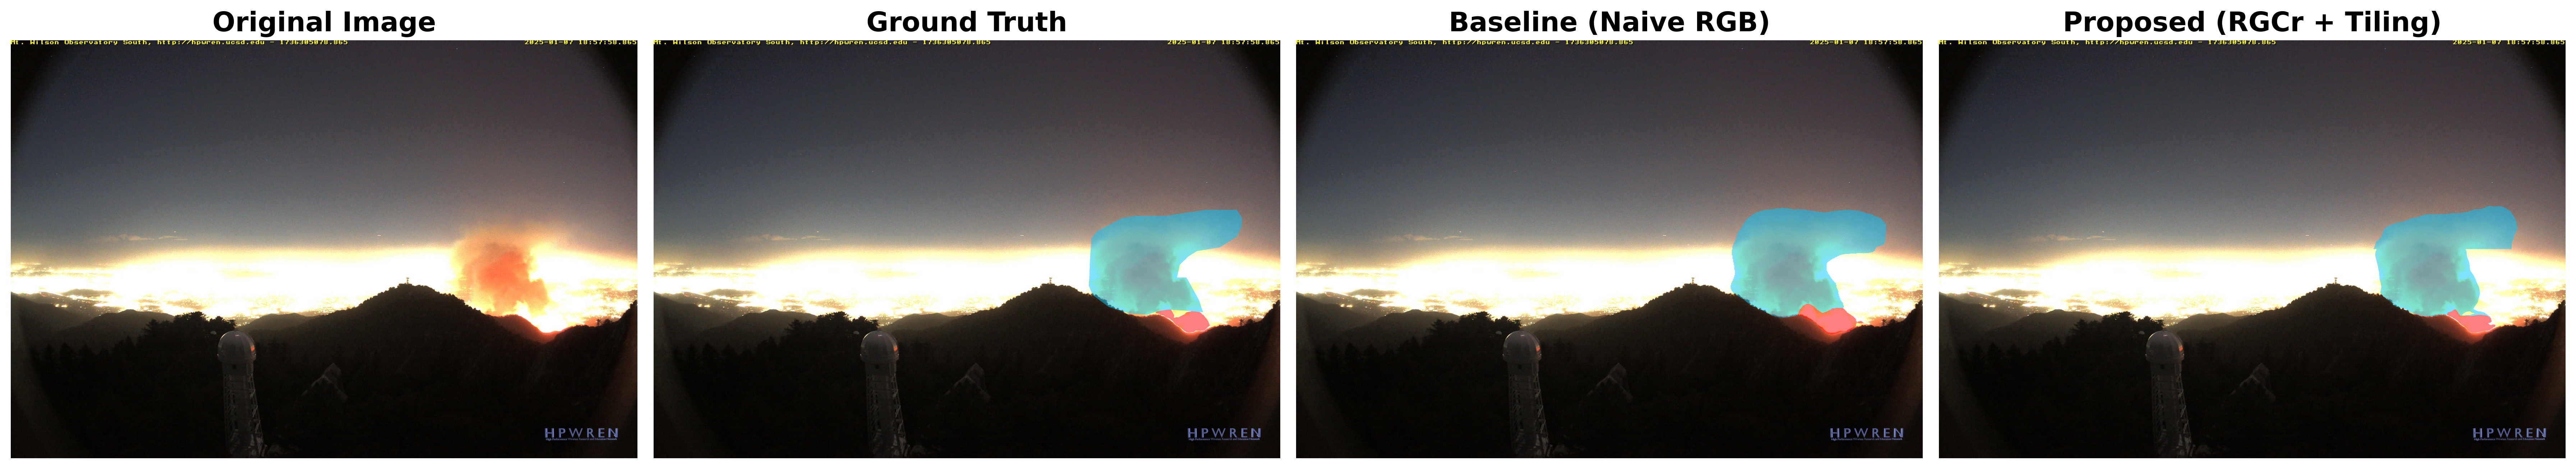
\includegraphics[width=\textwidth]{Figure_2_Qualitative_Comparison.png}}
\caption{Qualitative comparison of segmentation results on the FIgLib test set. From left to right: (a) Original high-resolution image; (b) Ground Truth annotations highlighting smoke (cyan) and fire (red); (c) Predictions from the Naive Baseline model; (d) Predictions from the Proposed Pipeline. The baseline model successfully detects the fire but severely over-predicts its boundaries, resulting in a highly imprecise and broad segmentation. In contrast, the proposed combined loss and data pipeline allow the PIDNet-M architecture to tightly and accurately delineate the exact boundaries of the minority combustion features.}
\label{fig:qualitative}
\end{figure*}

\section{Conclusion and Future Works}
In this paper, we proved that architectural efficiency must be paired with aggressive data and loss optimization to succeed in extreme environments. We demonstrated that a standard PIDNet-M architecture catastrophically fails on the minority Fire class (62.1\% mIoU) when faced with a 1:7 class imbalance. By introducing a custom Lovasz-Focal-Dice Combined Loss, we rescued the minority class performance to 79.9\%. Furthermore, by integrating a Balanced SAHI-style Tiling algorithm and an RGCr color space transformation, our proposed pipeline successfully pushed the Fire mIoU to a state-of-the-art 81.14\%. Overall, our methodology delivers an absolute performance increase of over 19\% compared to the standard baseline. These results definitively prove that data-centric tuning is just as critical as structural network design for the real-world deployment of life-safety surveillance systems.

\section*{Code Availability}
The source code, pre-trained models, and data splits used in this study are available at: \url{https://github.com/YourUsername/YourRepository}.

\begin{thebibliography}{00}
\bibitem{muhammad2023fire} I. Muhammad, F. Sthevanie, and K. N. Ramadhani, ``Fire Detection using Combined Approach of HSV-based Harris Corner Region Extraction and Vision Transformer Classification,'' in \textit{2023 International Conference on Data Science and Its Applications (ICoDSA)}, IEEE, 2023, pp. 117-122.
\bibitem{pidnet} J. Xu, Z. Xiong, S. P. Bhattacharyya, ``PIDNet: A Real-time Semantic Segmentation Network Inspired by PID Controllers,'' in \textit{Proceedings of the IEEE/CVF Conference on Computer Vision and Pattern Recognition (CVPR)}, 2023, pp. 19529-19539.
\bibitem{sahi} F. C. Akyon, S. O. Altinuc, and A. Temizel, ``Slicing Aided Hyper Inference and Fine-tuning for Small Object Detection,'' in \textit{2022 IEEE International Conference on Image Processing (ICIP)}, 2022, pp. 966-970.
\bibitem{focal} T. -Y. Lin, P. Goyal, R. Girshick, K. He, and P. Dollár, ``Focal Loss for Dense Object Detection,'' in \textit{IEEE Transactions on Pattern Analysis and Machine Intelligence}, vol. 42, no. 2, pp. 318-327, Feb. 2020.
\bibitem{lovasz} M. Berman, A. Rannen Triki, and M. B. Blaschko, ``The Lovász-Softmax loss: A tractable surrogate for the optimization of the intersection-over-union measure in neural networks,'' in \textit{Proceedings of the IEEE Conference on Computer Vision and Pattern Recognition (CVPR)}, 2018, pp. 4413-4421.
\bibitem{salehi2017tversky} S. S. M. Salehi, D. Erdogmus, and A. Gholipour, ``Tversky loss function for image segmentation using 3D fully convolutional deep networks,'' in \textit{International Workshop on Machine Learning in Medical Imaging}, Springer, 2017, pp. 379-387.
\bibitem{he2009imbalanced} H. He and E. A. Garcia, ``Learning from imbalanced data,'' in \textit{IEEE Transactions on Knowledge and Data Engineering}, vol. 21, no. 9, pp. 1263-1284, Sept. 2009.
\bibitem{buda2018systematic} M. Buda, A. Maki, and M. A. Mazurowski, ``A systematic study of the class imbalance problem in convolutional neural networks,'' in \textit{Neural Networks}, vol. 106, pp. 249-259, 2018.
\bibitem{wu2019adaframe} Z. Wu, C. Shen, and A. van den Hengel, ``AdaFrame: Adaptive Frame Selection for Fast Video Recognition,'' in \textit{Proceedings of the IEEE/CVF Conference on Computer Vision and Pattern Recognition (CVPR)}, 2019, pp. 1278-1287.
\bibitem{drummond2003c4} C. Drummond and R. C. Holte, ``C4.5, class imbalance, and cost updating: an empirical study,'' in \textit{ICML Workshop on Learning from Imbalanced Datasets}, 2003.
\bibitem{govil2020preliminary} K. Govil, M. L. Welch, J. T. Epstein, and J. K. MacAlpine, ``Preliminary results from a wildfire detection system using deep learning on remote camera images,'' in \textit{Remote Sensing}, vol. 12, no. 1, p. 166, 2020.
\bibitem{nguyen2023smokeynet} T. Nguyen, J. H. Park, A. Mai, D. W. O'Brien, and I. Altintas, ``SmokeyNet: Multimodal Wildland Fire Smoke Detection,'' in \textit{Remote Sensing}, vol. 15, no. 11, p. 2883, 2023.
\end{thebibliography}

\end{document}
